\section{Kristalle}
Eine nicht allzu häufig gestellte Frage ist, wie ein Kristall definiert ist.
Um zu klären, was ein Kristall mit Symmetrien zu tun hat, ist jedoch genau diese Frage äusserst relevant. 
Glücklicherweise ist das Innere eines Kristalles relativ einfach definiert.
\begin{definition}[Kristall]
    Ein Kristall besteht aus Atomen, welche sich in einem Muster arrangieren, welches sich in drei Dimensionen periodisch wiederholt.
\end{definition}

\begin{figure}
    \centering
    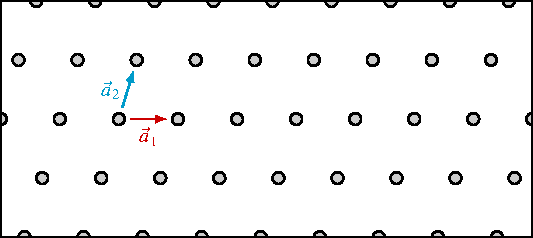
\includegraphics[]{papers/punktgruppen/figures/lattice}
    \caption{
        Zweidimensionales Kristallgitter.
        \label{fig:punktgruppen:lattice}
    }
\end{figure}
\subsection{Kristallgitter}
Ein zweidimensionales Beispiel eines solchen Muster ist Abbildung \ref{fig:punktgruppen:lattice}.
Für die Überschaubarkeit haben wir ein simples Motiv eines einzelnen grauen Punktes dargestellt und betrachten dies nur in zwei Dimensionen.
Die eingezeichneten Vektoren \(\vec{a}_1\) und \(\vec{a}_2\) sind die kleinstmöglichen Schritte im Raum bis sich das Kristallgitter wiederholt.
Wird ein beliebiger grauer Gitterpunkt in Abbildung \ref{fig:punktgruppen:lattice} gewählt und um eine ganzzahlige Linearkombination von \(\vec{a}_1\) und \(\vec{a}_2\) verschoben, endet er zwangsweise auf einem Gitterpunkt, wenn nicht wieder am selben Ort.
Im dreidimensionalen Raum können alle Gitterpunkte mit derselben Idee und einem zusätzlichen Vektor \(\vec{a}_3\) also
\[
  \vec{r} = n_1 \vec{a}_1 + n_2 \vec{a}_2 + n_3 \vec{a}_3 = \sum_i n_i \vec{a}_i
\]
erreicht werden sofern \(n_1,n_2,n_3 \in \mathbb{Z}\) sind.
Sind die Vektoren  \(\vec{a}_1\), \(\vec{a}_2\), \(\vec{a}_3\) gegeben, ist ein Kristallgitter eindeutig beschrieben, weswegen sie auch als Grundvektoren bekannt sind.

\subsection{Translationssymmetrie} 
Da sich das ganze Kristallgitter wiederholt, wiederholen sich auch dessen Eigenschaften periodisch mit den Grundvektoren.
Sollte man sich auf einem Gitterpunkt in einem Kristall aufhalten, ist es unmöglich zu wissen, auf welchem Gitterpunkt man sich befindet, da die Umgebungen aller Punkte identisch sind. 
Mit anderen Worten: Jedes Kristallgitter $ G $ ist \emph{translationssymmetrisch} in der Translation 
\[
    \vec{Q}_i(G) = G + \vec{a}_i,
\]
wobei der Vektor $\vec{a}_i$ ein Grundvektor sein muss.
Da die Translationssymmetrie beliebig oft mit allen Grundvektoren angewendet werden kann, 
können wir auch sagen, dass alle Verschiebungen um eine Linearkombination 
der Vektoren $\vec{a}_1$ , $\vec{a}_2$ und $\vec{a}_3$ erlaubt sind.
Dabei sollte erwähnt werden, dass eine Translationssymmetrie nur in unendlich grossen Kristallgittern besteht.

\subsection{Einschränkungen durch Kristallsymmetrien} \label{sec:punktgruppen:Translationssymmetrie}
 Die Translationssymmetrie ist wohl keine grosse Überraschung, wenn man die Abbildung \ref{fig:punktgruppen:lattice} betrachtet.
 Was nicht direkt ersichtlich ist, ist dass bei beliebigen Grundvektoren nicht beliebige Symmetrien erstellt werden können.
 Dies weil die Translationssymmetrie eines Kristalles weitere Symmetrien deutlich einschränkt.
  
\begin{figure}
    \centering
    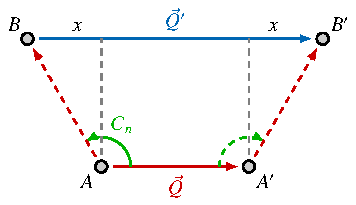
\includegraphics[]{papers/punktgruppen/figures/combine-symmetries}
    \caption{
        Translations und Rotationssymmetrisches Kristallgitter
    }
    \label{fig:punktgruppen:rot-geometry}
\end{figure}

\begin{satz} \label{thm:punktgruppen:crystal-restriction}
   Die Rotationssymmetrien eines Kristalls sind auf 2-fach, 3-fach, 4-fach und 6-fach beschränkt.
   Mit anderen Worten: Es sind nur Drehwinkel von
    0\(^{\circ}\),
    60\(^{\circ}\),
    90\(^{\circ}\),
    120\(^{\circ}\) und
    180\(^{\circ}\)
   m\"oglich.
\end{satz}

\begin{proof}
 In Abbildung \ref{fig:punktgruppen:rot-geometry} sehen wir Gitterpunkte und deren Zusammenhänge.

 \begin{itemize}
     \item  \(A\) ist unser erster Gitterpunkt. 

     \item  \(A'\) ist gegeben, weil wir \(A\) mit der Translation \(\vec{Q}\) um einen Grundvektor verschieben und wir wissen, 
            dass nach einer Translation wieder ein Gitterpunkt an der verschobenen Stelle sein muss.
     \item \(B\) entsteht, weil wir die Rotationssymmetrie \(C_n\) auf den Punkt \(A\) anwenden.
         Dadurch dreht sich das ganze Gitter um den Winkel \(360^\circ/n\). 
         Für uns bedeutet dies lediglich, dass unser zweiter Punkt \(A'\) abgedreht wird.
         An der neuen Position \(B\) von \(A'\) muss also auch ein Punkt des Gitters sein, um die Rotationssymmetrie zu erfüllen.
     \item \(B\) ist unser Name für diesen neuen Punkt.
         Da auch die Eigenschaften des Kristallgitters periodisch mit dem Gitter sein müssen, dürfen wir \(C_n\) auch auf \(A'\) anwenden.
         Also wenden wir \(C_n^{-1}\) auch auf \(A'\) an. 
         Dies dreht \(A\) auf einen neuen Punkt.
     \item \(B'\) ist kein zufälliger Name für diesen neuen Punkt, denn wir wissen, dass zwischen allen Punkten eine Translationssymmetrie bestehen muss.
         Die  Translationssymmetrie zwischen \(B\) und \(B'\) ist hier als \(\vec{Q}'\) bezeichnet.
 \end{itemize}  
 Mit den gegebenen Punkten lassen sich geometrische Folgerungen ziehen.
 Wir beginnen, indem wir die Länge der Verschiebung \(|\vec{Q}| = Q\) setzen und \(|\vec{Q}'| = Q'\).
 Aus Abbildung \ref{fig:punktgruppen:rot-geometry} ist ersichtlich, dass \(Q' = Q + 2x\).
 Da \(\vec{Q}\) eine Translation um ein Grundvektor ist , muss \(\vec{Q}'\) ein ganzes Vielfaches von \(\vec{Q}\) sein.
 Demnach ist auch die Länge
 \[
    Q' = nQ = Q + 2x .
 \]
 Die Strecke \(x\) lässt sich auch mit Hilfe der Trigonometrie und dem angenommenen Rotationswinkel \(\alpha\) ausdrücken:
 \[
    nQ = Q + 2Q\sin(\alpha - \pi/2) .
 \]
 Wir können durch \(Q\), dividieren um unabhängig von der Läge des Grundvektors zu werden, was auch Sinn macht, 
 da eine Skalierung eines Kristalles seine Symmetrieeigenschaften nicht tangiert.
 Zusätzlich können wir den Sinusterm vereinfachen. Somit wird
 \[
	 n = 1 - 2\cos\alpha \quad\text{oder}\quad
     \alpha = \cos^{-1}\left(\frac{1-n}{2}\right).
 \]
 Dies schränkt die möglichen Rotationssymmetrien auf 
 \(
     \alpha \in \left\{ 0^\circ, 60^\circ, 90^\circ, 120^\circ, 180^\circ\right\}
 \)
ein.
\end{proof}

\begin{figure}
    \centering
    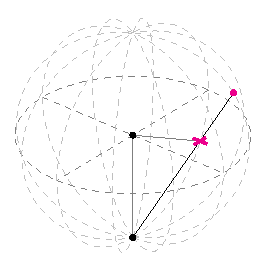
\includegraphics[height=6cm]{papers/punktgruppen/figures/stereographic-projections}
    \caption{
      Stereografische Projektion einer \(C_{i}\) Symmetrie. Es wird eine Linie vom magentafarbenen Punkt auf der oberen Hälfte der Kugel zum Südpol gezogen.
      Wo die Linie die Ebene schneidet (\(z = 0\)), ist die Projektion des Punktes.
      Die Koordinaten der Projektionen sind einfach zu berechnen: ein Punkt auf eine Kugel mit Radius \(r\) mit den Koordinaten \(x, y, z,\) wird auf \(xr/(r + z), yr/(r + z)\) projiziert.
      Für den orangefarbenen Punkt unterhalb des Äquators wird die Linie zum Nordpol gezogen und die Projektionsformel hat stattdessen einen Nenner von \(r - z\).
    }
    \label{fig:punktgruppen:stereographic-projections}
\end{figure}

\subsection{Kristallklassen}

Im vorausgegangenen Abschnitt wurde gezeigt, dass in einem zweidimensionalen Kristallgitter nicht alle Symmetrien möglich sind.
 Mit weiteren ähnlichen Überlegungen kann gezeigt werden, dass Kristalle im dreidimensionalen Raum nur auf genau 32 Arten rein punktsymmetrische Symmetriegruppen bilden können.
 Diese 32 möglichen Symmetriegruppen scheinen durchaus relevant zu sein, denn sie werden unter anderem als Kristallklassen bezeichnet.
 Die 32 möglichen Kristallklassen sind auf Abbildung \ref{fig:punktgruppen:kristallklassen} zu sehen.
 Die Darstellung von dreidimensionalen Punktsymmetrien wurde mit der stereographischen Projektion ermöglicht (siehe Abbildung \ref{fig:punktgruppen:stereographic-projections}), wobei die gestrichelten Klassen aus Gründen der Überschaubarkeit nicht im Detail gezeichnet wurden.


\begin{figure}
    \centering
    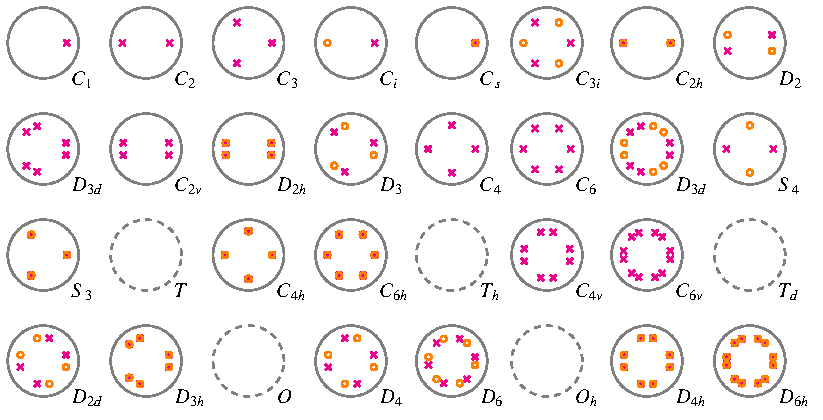
\includegraphics[]{papers/punktgruppen/figures/projections}
    \caption{Kristallklassen mit zugehörigem Schönflies-Symbol}
    \label{fig:punktgruppen:kristallklassen}
\end{figure}

\subsubsection{Schönflies-Symbolik}

Jede der 32 Kristallklassen auf der Abbildung \ref{fig:punktgruppen:kristallklassen} ist mit ihrem zugehörigen Schönflies-Symbol bezeichnet.
 Die Schönflies-Symbolik stammt von dem Mathematiker Arthur Moritz Schönflies, welcher sich unter anderem mit der Klasifizierung der Punktgruppen auseinandergesetzt hat.
 Er hat Untergruppen gebildet, welche als Grossbuchstaben in Abbildung \ref{fig:punktgruppen:kristallklassen} zu sehen sind.
 \begin{itemize}
   \item In Kristallen ist nur die Drehgruppe \(C\), Diedergruppe \(D\), Drehspiegelgruppe \(S\), Tetraedergruppe \(T\) und die Oktaedergruppe \(O\) zu finden.
	   Es gäbe auch die Ikosaedergruppe \(I\) und die Kugelgruppe \(K\), diese sind aber nach Satz \ref{thm:punktgruppen:crystal-restriction} nicht kompatibel mit der Translationssymmetrie eines Kristalles und daher in der Kristallographie nicht relevant.  
   \item Dank Abschnitt \ref{sec:punktgruppen:Translationssymmetrie} wissen wir, wieso in Abbildung \ref{fig:punktgruppen:kristallklassen} auf \(C\) nur ganz bestimmte Subskripte folgen.
     Ist im Subskript eine Zahl \(n\) zu finden, steht dies für eine \(n\)-fache Symmetrie.
     Daher darf \(C_5\) auf der Abbildung \ref{fig:punktgruppen:kristallklassen} nicht vorkommen, da \(360^\circ/5 =  72^\circ\) was nach Satz \ref{thm:punktgruppen:crystal-restriction} keine mögliche Rotationssymmetrie eines Kristalles ist.
   \item Sind im Subskript Buchstaben, definieren diese weitere Symmetrieeigenschaften der Klasse.
     Für die folgenden Betrachtungen müssen wir uns Abbildung \ref{fig:punktgruppen:kristallklassen} genauer ansehen.
     Dabei ist mit horizontal flach auf dem Papier gemeint.
     \begin{itemize}
       \item[\(h\)] bezeichnet eine horizontale Spiegelebene und 
       \item[\(v\)] eine Symmetrieebene, was eine Spiegelebene ist, die sich mit der Symmetrie mitdreht.
         Zum Beispiel hat \(C_{3v}\) eine vertikale Spiegelebene, die durch die 3-fache Drehsymmetrie als 3 Spiegelebenen erscheinen.
       \item[\(s\)] ist ein spezielles Subskript um die beiden Symmetriegruppen \(C_{1v}\) und \(C_{1h}\) zu beschreiben, weil \(C_{1v} = C_{1h}\).
       \item[\(d\)] symbolisiert eine diagonale Symmetrieebene.
         Es wird ersichtlich wie diagonal gemeint ist, wenn man \(D_2\) zu \(D_{2d}\) vergleicht.
       \item[\(i\)] steht für ein Inversionszentrum. Hat eine Symmetriegruppe ein Inversionszentrum, bedeutet dies dass sie im Ursprung punktsymmetrisch ist.
     \end{itemize}
 \end{itemize}
Zu beachten ist jedoch, dass manche Symmetriegruppen mit mehreren Schönflies-Symbolen beschieben werden können.
 \(C_{3i}\) beschreibt genau das selbe wie \(S_6\), da eine dreifache Rotationssymmetrie mit einem Inversionszentrum einer sechsfachen Drehspiegelsymmetrie entspricht.




%% vim:spell spelllang=de showbreak=.. breakindent linebreak:
